\documentclass[12pt,english]{article}
\usepackage[english]{babel}
\usepackage{graphicx}
\usepackage{amsmath}
\usepackage{adjustbox}
\usepackage{multirow}
\usepackage{subcaption}
\usepackage{amssymb}
\usepackage[hidelinks]{hyperref}
\usepackage{caption}
\usepackage{amsthm}
\usepackage{multicol}
\usepackage[outputdir=build]{minted}
\usepackage{float}
\usepackage{titling}
\usepackage{soul}
\usepackage{listings}
\usepackage{array}
\graphicspath{ {./img/}}
\selectlanguage{english}
\usepackage[nottoc]{tocbibind}
\usepackage[utf8]{inputenc}
\usepackage{graphicx}
\usepackage[a4paper,left=2cm,right=2cm,top=2.5cm,bottom=2.5cm]{geometry}
\RecustomVerbatimEnvironment{Verbatim}{BVerbatim}{}


\title{Media Informatic Systems}
\setlength{\droptitle}{10em}
\author{Carlos Sánchez Páez}

\makeindex
\begin{document}


\begin{titlepage}

\newlength{\centeroffset}
\setlength{\centeroffset}{-0.5\oddsidemargin}
\addtolength{\centeroffset}{0.5\evensidemargin}
\thispagestyle{empty}

\noindent\hspace*{\centeroffset}
\begin{minipage}{\textwidth}

\centering

\includegraphics[width=0.75\textwidth]{bme_logo.jpg}\\[1.4cm]

\textsc{ \Large Media Informatic Systems\\[4cm]}

\textsc{\Huge Image recognition task}\\[0.75cm]

{\Large\bfseries Final progress report\\}
\end{minipage}

\vspace{8cm}
\noindent\hspace*{\centeroffset}
\begin{minipage}{\textwidth}
\centering

\textbf{Author}\\ {Carlos Sánchez Páez}\\
\texttt{http://www.github.com/csp98}\\[0.5cm]
\textsc{Budapest University of Technology and Economics}\\
\vspace{1cm}
\textsc{Academic year 2018-2019}
\end{minipage}
\end{titlepage}
\thispagestyle{empty}
\newpage
\tableofcontents{}
\listoffigures
\thispagestyle{empty}
\newpage

\section{Description of the task}

My task consists on the development of a neural net which will be able to classify different types of RGB images according to the used dataset.

\section{Dataset}

The train and test images will be taken from \emph{CIFAR100}. It is a dataset which contains 50,000 32x32 color training images, labeled over 100 categories, and 10,000 test images. \\

The main advantage of this dataset is that it is included in the \textit{keras} dataset. This allows us to load the data by just executing this sentences:

\begin{figure}[H]
\centering
\begin{minted}[linenos=true,breaklines=true,tabsize=2]{python}
from keras.datasets import cifar100
(x_train, y_train), (x_test, y_test) = cifar100.load_data()
\end{minted}
\caption{Loading the CIFAR100 dataset}
\end{figure}

\section{Diary of work}

\begin{enumerate}
	\item \textbf{Familiarize with \emph{TensorFlow}}. The first thing I did was reading some \emph{TensorFlow} tutorials. Specifically, I developed a classifier which was able to distinguish between dogs and cats with the help of a tutorial. 
	\item \textbf{Try to adapt the algorithm}. I thought about converting the dogs and cats classifier into a biger one, so I made the corresponding changes to use it with the \emph{Caltech-101} dataset. The main problem was that the number of images was too low for some categories. That is why I only achieved a 34.5\% success rate.
	\item \textbf{Jump to Caltech-256}. As there were too few images in Caltech-101, I downloaded the Caltech-256 dataset and started to work with it. But I had the opposite problem: as there were too much images, my local PC memory was not enough. To fix this, I created a virtual machine using Google Cloud (30GB of RAM). After 8 hours of training, the accuracy that I achieved was  0.39\%. That is because the images for the categories were too similar and I did not apply any preprocessing.
	\item \textbf{Decide to work with \emph{Caltech-101} and local PC}. As the results obtained in \emph{Caltech-256} were not good, I decided to center myself on \emph{Caltech-101}.
	\item \textbf{Jump to \emph{Keras}}. In class, we saw a \emph{Keras} example. As I could see, the code was much more readable and easy to understand, so I started to recode the program using \emph{Keras} and \emph{Python 3.6}.
	\item \textbf{Error with shapes}. I had a lot of problems with the input shapes of my images (I was importing local files directly to the program). I spent here more than a week trying to figure out the error. 
	\item \textbf{Dataset change}. Tired of spending time on the shape error, I decided to use the \emph{CIFAR100} dataset because the loading functions were already implemented.
	\item \textbf{Parameters calibration}. I modified some parameters to make the model better, such as \emph{batch size} and \emph{preprocessing functions}.
\end{enumerate}

\section{Preprocessing of the images}

To preprocess the images I use the \emph{ImageDataGenerator} Keras utility. It randomly flips, applies filters, etc. to the images so that the input data is more varied. The parameters used are the following:

\begin{figure}[H]
\centering
\begin{minted}[linenos=true,breaklines=true,tabsize=2]{python}
datagen = ImageDataGenerator(
    featurewise_center=False,  
    samplewise_center=False,  
    featurewise_std_normalization=False,  
    samplewise_std_normalization=False, 
    zca_whitening=False,  
    rotation_range=0,
    width_shift_range=0.1,
    height_shift_range=0.1,
    horizontal_flip=True,  
    vertical_flip=True) 
\end{minted}
\caption{Preprocessing of the images.}
\end{figure}

\section{Structure of the neural net}

\begin{itemize}
	\item Two convolutional layers with 128 filters using the ELU activation function.
	\item A pooling layer to reduce the size of the images.
	\item Two convolutional layers with 256 filters using the ELU activation function.
	\item A dropout layer to prevent from overfitting.
	\item Two convolutional layers with 512 filters using the ELU activation function.
	\item Another dropout layer.
	\item A flatten layer to convert the result to 1D.
	\item A fully connected layer.
	\item Another dropout.
	\item The output layer with 100 neurons, one for each class. The used activation function is softmax.
\end{itemize}

The optimizer that the model uses is \emph{RMSProp}, with a learning rate of 0.0001. The batch size is 64.

\begin{figure}[H]
\centering
\begin{minted}[linenos]{python}
model = Sequential()

model.add(Conv2D(128, (3, 3), padding='same',
                 input_shape=x_train.shape[1:], activation='elu'))
model.add(Conv2D(128, (3, 3), activation='elu'))
model.add(MaxPooling2D(pool_size=(2, 2)))
model.add(Dropout(0.25))

model.add(Conv2D(256, (3, 3), padding='same', activation='elu'))
model.add(Conv2D(256, (3, 3), activation='elu'))
model.add(MaxPooling2D(pool_size=(2, 2)))
model.add(Dropout(0.25))

model.add(Conv2D(512, (3, 3), padding='same', activation='elu'))
model.add(Conv2D(512, (3, 3), activation='elu'))
model.add(MaxPooling2D(pool_size=(2, 2)))
model.add(Dropout(0.25))


model.add(Flatten())
model.add(Dense(1024, activation='elu'))
model.add(Dropout(0.5))
model.add(Dense(parameters.NUM_CLASSES, activation='softmax'))

\end{minted}
\caption{Build of the net}
\end{figure}

\newpage

\section{The final state of the model}

First, I trained the model with 200 epochs so that I could find the global maximum of the test accuracy. It took more than 8 hours on my local PC, but the results were quite good:

\begin{figure}[H]
\centering
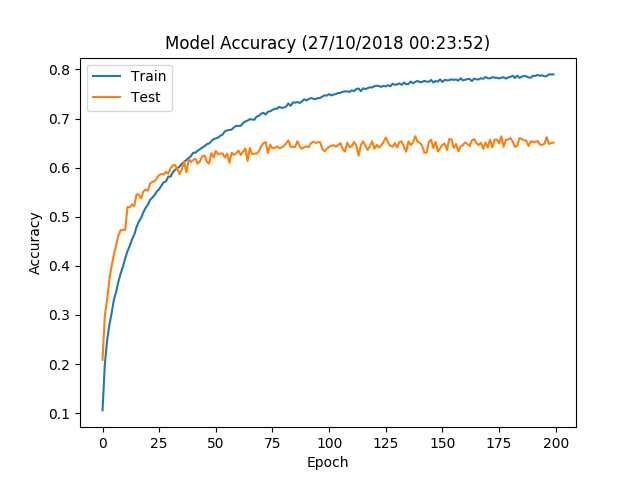
\includegraphics[scale=0.85]{accuracy.png}
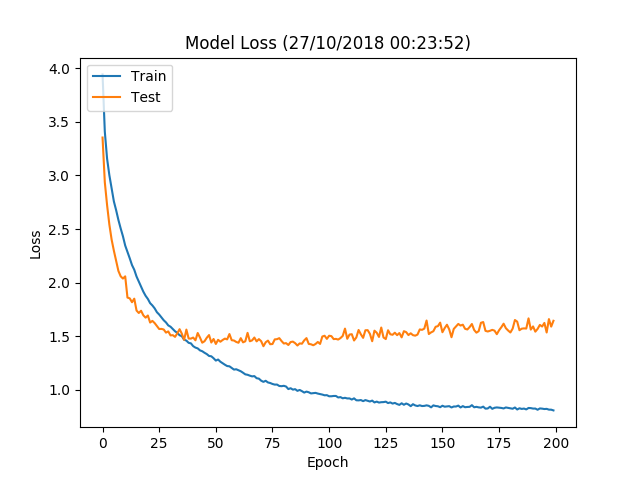
\includegraphics[scale=0.85]{loss.png}
\caption{Accuracy and loss of the model (200 epochs)}
\end{figure}

We can see that the accuracy is around 60\%. Concretely, the maximum accuracy was 68.77\%, reached on epoch 139.\\

With those results, I re-trained the model. It took 3:30 hours and the results were the following:

\begin{figure}[H]
\centering
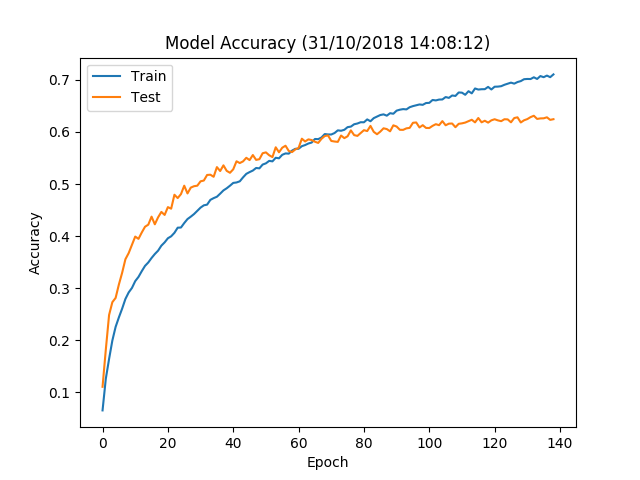
\includegraphics[scale=0.85]{accuracy_139.png}
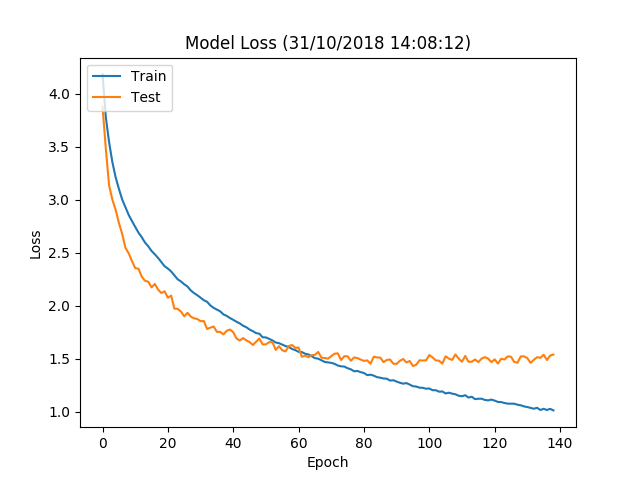
\includegraphics[scale=0.85]{loss_139.png}
\caption{Accuracy and loss of the model (139 epochs)}
\end{figure}


\section{Examples}
Let's run the model with different images retrieved from the Internet so that we can see its behaviour.

\begin{figure}[H]
\centering
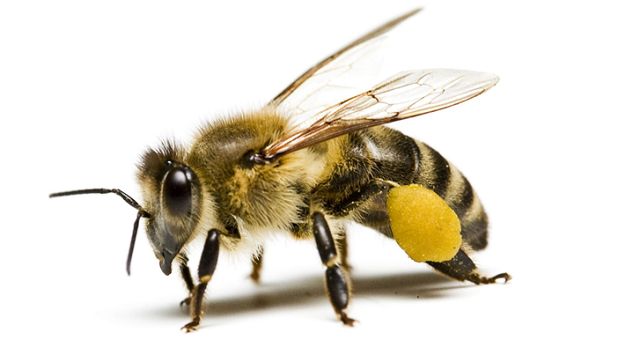
\includegraphics[scale=0.27]{bee.png}
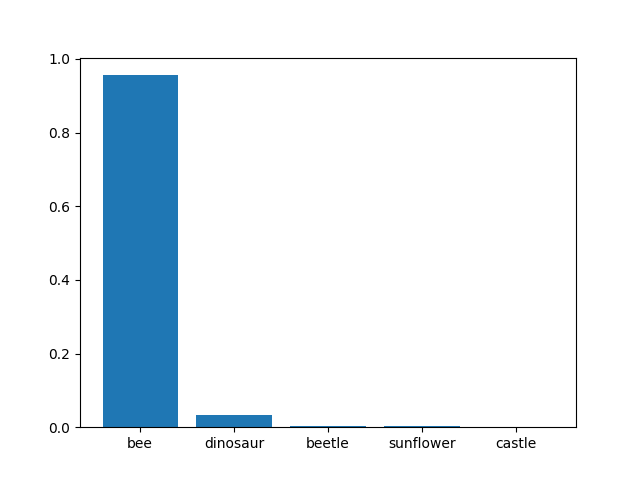
\includegraphics[scale=0.75]{bee_prediction.png}
\caption{Bee prediction}
\end{figure}


\begin{figure}[H]
\centering
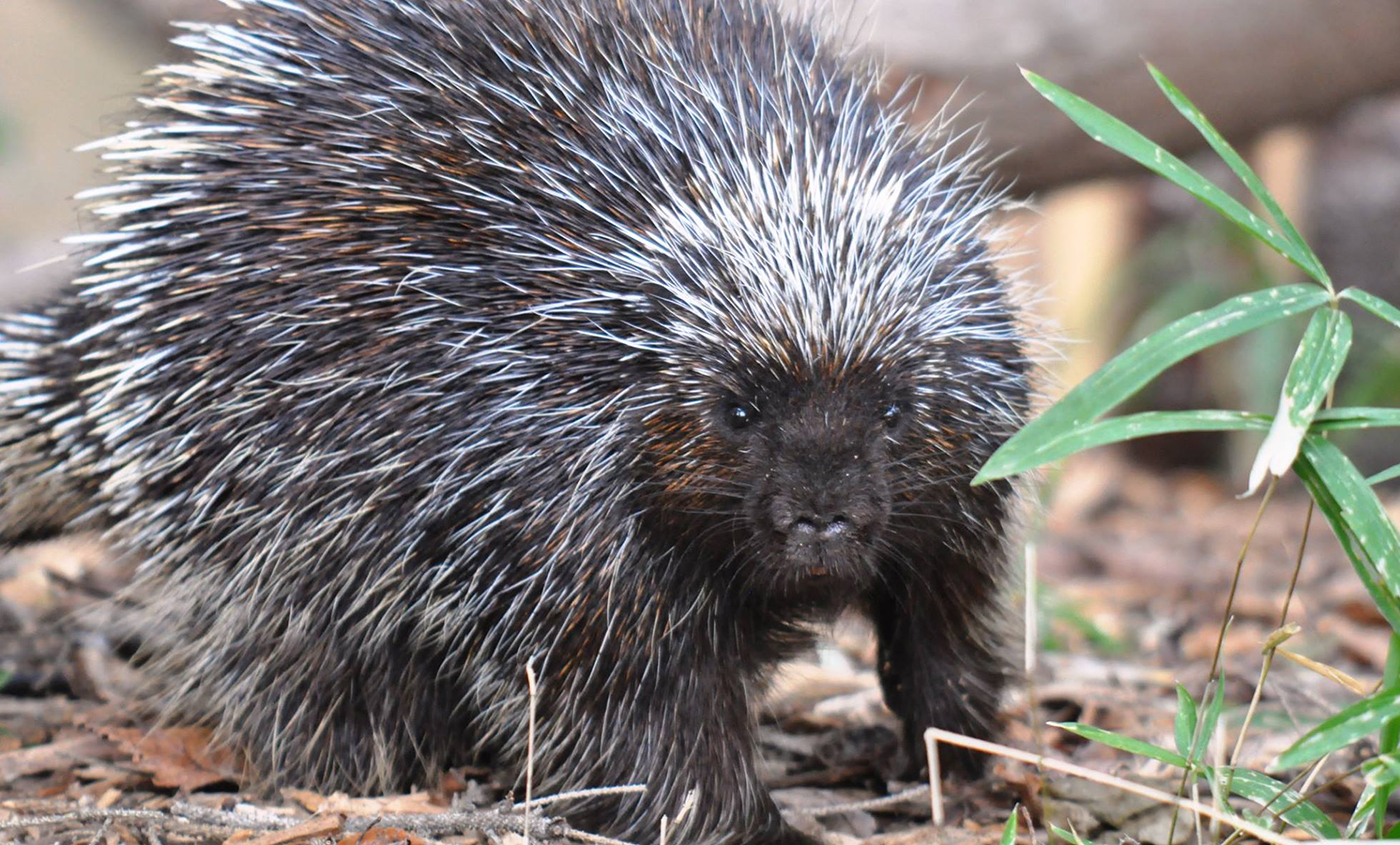
\includegraphics[scale=0.35]{porcupine.jpg}
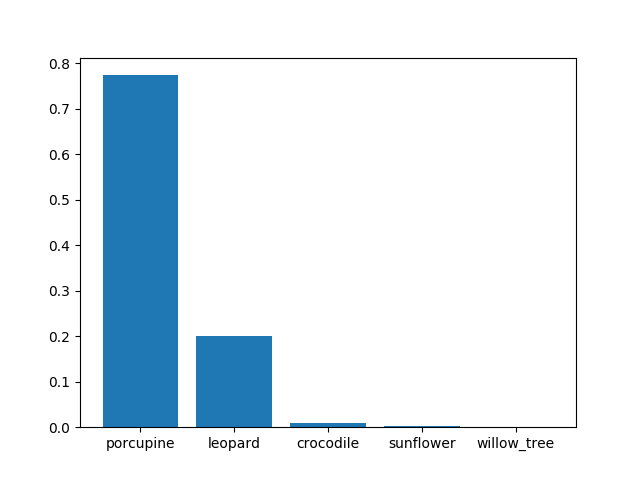
\includegraphics[scale=0.75]{porcupine_prediction.png}
\caption{Porcupine prediction}
\end{figure}

\begin{figure}[H]
\centering
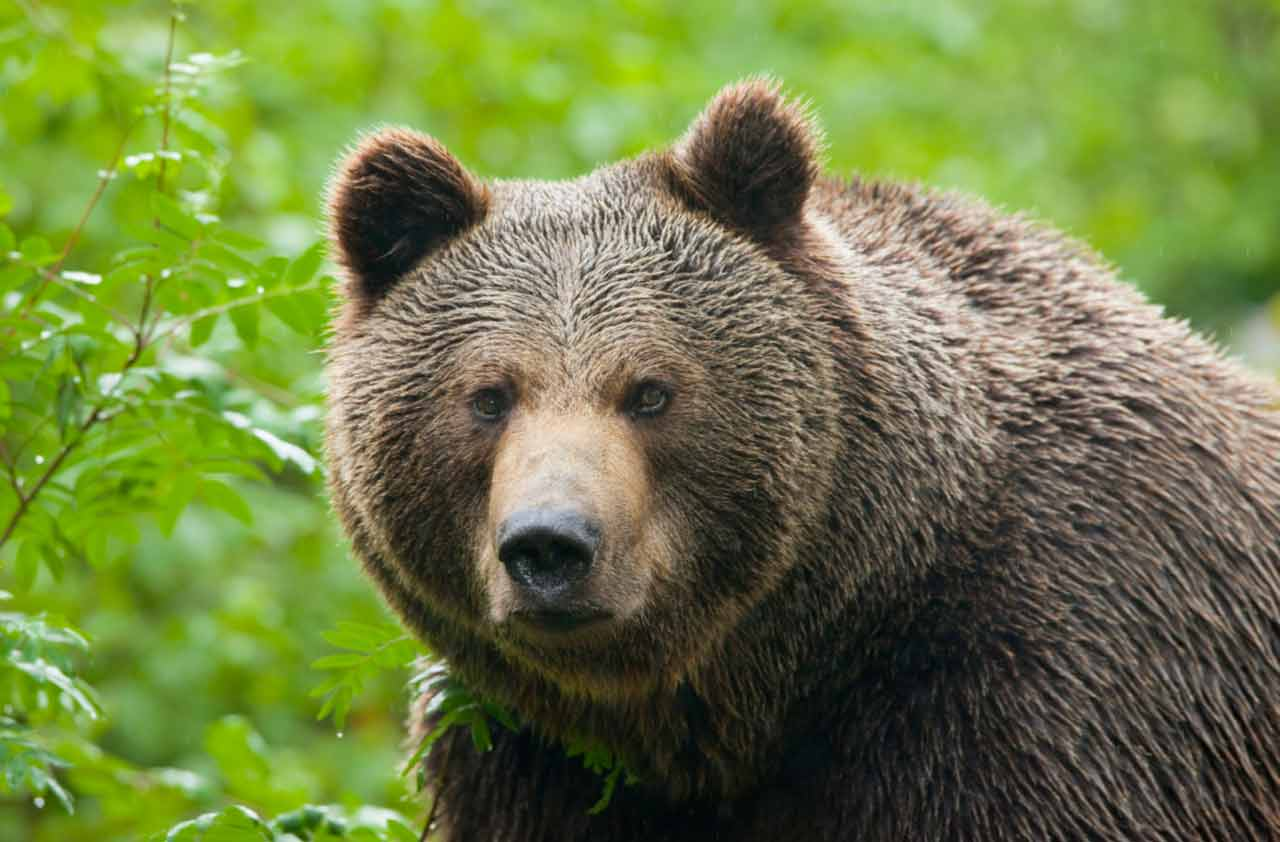
\includegraphics[scale=0.1]{bear.jpg}
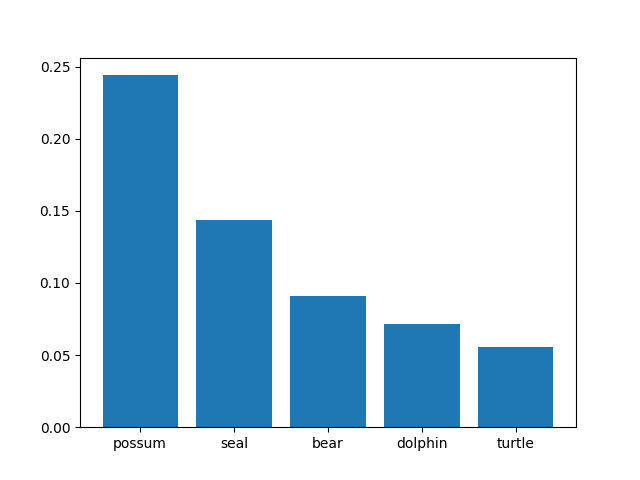
\includegraphics[scale=0.75]{bear_prediction.png}
\caption{Bear prediction}
\end{figure}

\begin{figure}[H]
\centering
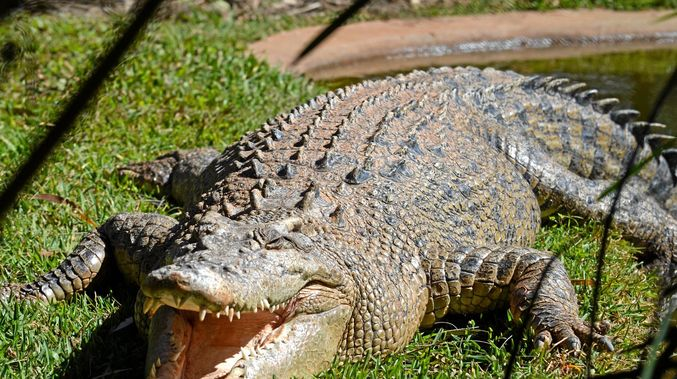
\includegraphics[scale=0.15]{crocodile.jpg}
\hspace{2em}
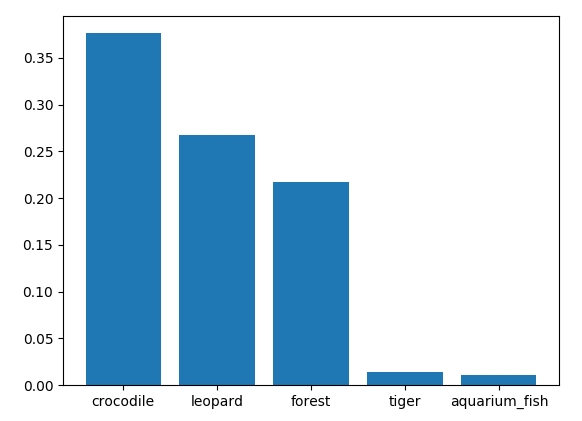
\includegraphics[scale=0.5]{crocodile_prediction.jpg}
\caption{Crocodile prediction}
\end{figure}

\newpage

\section{Annex: classes contained in the dataset}
\begin{multicols}{3}
\begin{enumerate}
\item apple
\item aquarium\_fish
\item baby
\item bear
\item beaver
\item bed
\item bee
\item beetle
\item bicycle
\item bottle
\item bowl
\item boy
\item bridge
\item bus
\item butterfly
\item camel
\item can
\item castle
\item caterpillar
\item cattle
\item chair
\item chimpanzee
\item clock
\item cloud
\item cockroach
\item couch
\item crab
\item crocodile
\item cup
\item dinosaur
\item dolphin
\item elephant
\item flatfish
\item forest
\item fox
\item girl
\item hamster
\item house
\item kangaroo
\item keyboard
\item lamp
\item lawn\_mower
\item leopard
\item lion
\item lizard
\item lobster
\item man
\item maple\_tree
\item motorcycle
\item mountain
\item mouse
\item mushroom
\item oak\_tree
\item orange
\item orchid
\item otter
\item palm\_tree
\item pear
\item pickup\_truck
\item pine\_tree
\item plain
\item plate
\item poppy
\item porcupine
\item possum
\item rabbit
\item raccoon
\item ray
\item road
\item rocket
\item rose
\item sea
\item seal
\item shark
\item shrew
\item skunk
\item skyscraper
\item snail
\item snake
\item spider
\item squirrel
\item streetcar
\item sunflower
\item sweet\_pepper
\item table
\item tank
\item telephone
\item television
\item tiger
\item tractor
\item train
\item trout
\item tulip
\item turtle
\item wardrobe
\item whale
\item willow\_tree
\item wolf
\item woman
\item worm
\end{enumerate}
\end{multicols}


\begin{thebibliography}{9}

\bibitem{Keras documentation} 
Keras documentation
\\\texttt{https://keras.io/}

\bibitem{Moodle} 
Moodle
\\\texttt{https://elearning.tmit.bme.hu/login/index.php}

\bibitem{Tensorflow Tutorial} 
Tensorflow Tutorial
\\\texttt{https://cv-tricks.com/tensorflow-tutorial/training-convolutional\\-neural-network-for-image-classification/}

\bibitem{Some Datasets} 
Some Datasets
\\\texttt{https://www.analyticsvidhya.com/blog/2018/03/\\comprehensive-collection-deep-learning-datasets/}


\bibitem{Understanding Convolutions} 
Understanding Convolutions
\\\texttt{https://towardsdatascience.com/intuitively-understanding\\-convolutions-for-deep-learning-1f6f42faee1}

\bibitem{Deep neural net tutorial} 
Deep neural net tutorial
\\\texttt{https://medium.com/@tifa2up/image-classification\\-using-deep-neural-networks-a-beginner-friendly-\\approach-using-tensorflow-94b0a090ccd4}

\bibitem{Caltech-101 dataset} 
Caltech-101 dataset
\\\texttt{http://www.vision.caltech.edu/Image\_Datasets/Caltech101/}


\bibitem{Caltech-256 dataset} 
Caltech-256 dataset
\\\texttt{http://www.vision.caltech.edu/Image\_Datasets/Caltech256/}


\bibitem{TensorFlow tutorial} 
TensorFlow tutorial
\\\texttt{https://cv-tricks.com/artificial-intelligence/deep-learning\\/deep-learning-frameworks/tensorflow/tensorflow-tutorial/}

\bibitem{Basic classification tutorial with Tensorflow} 
Basic classification tutorial with Tensorflow
\\\texttt{https://www.tensorflow.org/tutorials/keras/basic\_classification}


\bibitem{Keras tutorial} 
Keras tutorial
\\\texttt{https://medium.com/@vijayabhaskar96/tutorial-image-classification\\-with-keras-flow-from-directory-and-generators-95f75ebe5720}

\bibitem{Another Keras tutorial} 
Another Keras tutorial
\\\texttt{https://machinelearningmastery.com/tutorial-\\first-neural-network-python-keras/}

\bibitem{Doubts resolution} 
Doubts resolution
\\\texttt{https://stackoverflow.com/}

\end{thebibliography}



\end{document}